%=======================02-713 LaTeX template, following the 15-210 template==================
%
% You don't need to use LaTeX or this template, but you must turn your homework in as
% a typeset PDF somehow.
%
% How to use:
%    1. Update your information in section "A" below
%    2. Write your answers in section "B" below. Precede answers for all 
%       parts of a question with the command "\question{n}{desc}" where n is
%       the question number and "desc" is a short, one-line description of 
%       the problem. There is no need to restate the problem.
%    3. If a question has multiple parts, precede the answer to part x with the
%       command "\part{x}".
%    4. If a problem asks you to design an algorithm, use the commands
%       \algorithm, \correctness, \runtime to precede your discussion of the 
%       description of the algorithm, its correctness, and its running time, respectively.
%    5. You can include graphics by using the command \includegraphics{FILENAME}
%
\documentclass[11pt]{article}
\usepackage{amsmath,amssymb,amsthm}
\usepackage{graphicx}
\usepackage[margin=1in]{geometry}
\usepackage{fancyhdr}
\usepackage{listings}
\setlength{\parindent}{0pt}
\setlength{\parskip}{5pt plus 1pt}
\setlength{\headheight}{13.6pt}
\newcommand\question[2]{\vspace{.25in}\hrule\textbf{#1: #2}\vspace{.5em}\hrule\vspace{.10in}}
\renewcommand\part[1]{\vspace{.10in}\textbf{(#1)}}
\newcommand\algorithm{\vspace{.10in}\textbf{Algorithm: }}
\newcommand\correctness{\vspace{.10in}\textbf{Output: }}
\newcommand\runtime{\vspace{.10in}\textbf{Running time: }}
\pagestyle{fancyplain}
\lhead{\textbf{\NAME\ (\ANDREWID)}}
\chead{\textbf{Lab\HWNUM}}
\rhead{\today}
\begin{document}\raggedright
%Section A==============Change the values below to match your information==================
\newcommand\NAME{Yao Xiao}  % your name
\newcommand\ANDREWID{2019180015}     % your andrew id
\newcommand\HWNUM{3}              % the homework number
%Section B==============Put your answers to the questions below here=======================

% no need to restate the problem --- the graders know which problem is which,
% but replacing "The First Problem" with a short phrase will help you remember
% which problem this is when you read over your homeworks to study.

\question{1}{The First Problem} 

\part{a} \algorithm
\begin{lstlisting}
import numpy as np
 
def tanh(x):
    return np.tanh(x)
 
def tanh_deriv(x):
    return 1.0 - np.tanh(x) * np.tanh(x)

class MLP:
    def __init__(self, layers):
        self.layers = layers
        self.activation = tanh
        self.activation_deriv = tanh_deriv
        self.num_layers = len(layers)
        self.bias = [np.random.randn(x) for x in layers[1:]]
        self.weights = [np.random.randn(y, x) for x, y in zip(layers[:-1], layers[1:])]
 
    def fit(self, X, y, learning_rate, epochs):
        for k in range(epochs):
            for i in range(len(X)):
                #store to use
                results = [X[i]]
                for b, w in zip(self.bias, self.weights):
                    z = np.dot(w, results[-1])+b
                    output = self.activation(z)
                    results.append(output)

                error = y[i] - results[-1]
                deltas = [error * self.activation_deriv(results[-1])]
 
                for l in range(self.num_layers-2, 0, -1):
                    deltas.append(self.activation_deriv(results[l]) * np.dot( deltas[-1],self.weights[l]))

                deltas.reverse()
           
                for j in range(self.num_layers-1):
                    layers = np.array(results[j])
                    delta_w = learning_rate * ((np.atleast_2d(deltas[j]).T).dot(np.atleast_2d(layers)))
                    self.weights[j] += delta_w
                    delta_t = learning_rate * deltas[j]
                    self.bias[j] += delta_t
 
    def predict(self, x):
        for b, w in zip(self.bias, self.weights):
            z = np.dot(w, x) + b
            x = self.activation(z)
        return x


mlp = MLP([2,4,3,1])
X = np.array([[0, 1], [1, 0], [0, 0], [1, 1]])
y = np.array([1, 1, 0, 0])
mlp.fit(X, y, 0.05, epochs=1000)
for i in [[0, 1], [1, 0], [0, 0], [1, 1]]:
  print(i, mlp.predict(i))
\end{lstlisting}

\part{b} \correctness\\
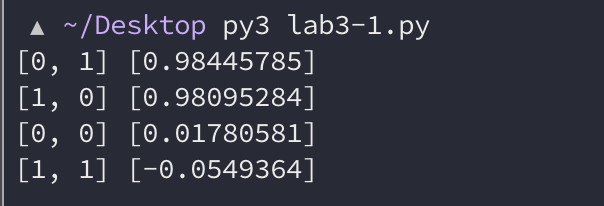
\includegraphics[scale=1]{ot1.png}

\question{2}{The Second Problem} 
\part{a} \algorithm
\begin{lstlisting}
import csv
import random
import math
random.seed(250)

with open('iris.csv') as csvfile:
    csvreader = csv.reader(csvfile)
    next(csvreader, None)
    dataset = list(csvreader)

for row in dataset:
    row[4] = ["Iris-setosa", "Iris-versicolor", "Iris-virginica"].index(row[4])
    row[:4] = [float(row[j]) for j in range(len(row))]

random.shuffle(dataset)
datatrain = dataset[:int(len(dataset) * 0.8)]
datatest = dataset[int(len(dataset) * 0.8):]
train_X = [data[:4] for data in datatrain]
train_y = [data[4] for data in datatrain]
test_X = [data[:4] for data in datatest]
test_y = [data[4] for data in datatest]


def matrix_mul_bias(A, B, bias):
    C = [[0 for i in range(len(B[0]))] for i in range(len(A))]    
    for i in range(len(A)):
        for j in range(len(B[0])):
            for k in range(len(B)):
                C[i][j] += A[i][k] * B[k][j]
            C[i][j] += bias[j]
    return C

def vec_mat_bias(A, B, bias): 
    C = [0 for i in range(len(B[0]))]
    for j in range(len(B[0])):
        for k in range(len(B)):
            C[j] += A[k] * B[k][j]
            C[j] += bias[j]
    return C


def mat_vec(A, B):
    C = [0 for i in range(len(A))]
    for i in range(len(A)):
        for j in range(len(B)):
            C[i] += A[i][j] * B[j]
    return C

def sigmoid(A, deriv=False):
    if deriv:
        for i in range(len(A)):
            A[i] = A[i] * (1 - A[i])
    else:
        for i in range(len(A)):
            A[i] = 1 / (1 + math.exp(-A[i]))
    return A


alfa = 0.005
epoch = 2000
# [input layer:feature of Iris, hidden layer, output layer:class of Iris]
neuron = [4, 4, 3] 
weight = [[0 for j in range(neuron[1])] for i in range(neuron[0])]
weight_2 = [[0 for j in range(neuron[2])] for i in range(neuron[1])]
bias = [0 for i in range(neuron[1])]
bias_2 = [0 for i in range(neuron[2])]

for i in range(neuron[0]):
    for j in range(neuron[1]):
        weight[i][j] = 2 * random.random() - 1

for i in range(neuron[1]):
    for j in range(neuron[2]):
        weight_2[i][j] = 2 * random.random() - 1


for e in range(epoch):
    cost_total = 0
    for idx, x in enumerate(train_X):
        
        h_1 = vec_mat_bias(x, weight, bias)
        X_1 = sigmoid(h_1)
        h_2 = vec_mat_bias(X_1, weight_2, bias_2)
        X_2 = sigmoid(h_2)
    
        target = [0, 0, 0]
        target[int(train_y[idx])] = 1

        eror = 0
        for i in range(neuron[2]):
            eror +=  (target[i] - X_2[i]) ** 2 
        cost_total += eror * 1 / neuron[2]

        delta_2 = []
        for j in range(neuron[2]):
            delta_2.append(-1 * 2. / neuron[2] * (target[j]-X_2[j]) * X_2[j] * (1-X_2[j]))

        for i in range(neuron[1]):
            for j in range(neuron[2]):
                weight_2[i][j] -= alfa * (delta_2[j] * X_1[i])
                bias_2[j] -= alfa * delta_2[j]
        
        delta_1 = mat_vec(weight_2, delta_2)
        for j in range(neuron[1]):
            delta_1[j] = delta_1[j] * (X_1[j] * (1-X_1[j]))
        
        for i in range(neuron[0]):
            for j in range(neuron[1]):
                weight[i][j] -=  alfa * (delta_1[j] * x[i])
                bias[j] -= alfa * delta_1[j]

    cost_total /= len(train_X)
    if(e % 100 == 0):
        print(cost_total)


#Test
result = matrix_mul_bias(test_X, weight, bias)
output = matrix_mul_bias(result, weight_2, bias)

predict = []
for r in output:
    predict.append(max(enumerate(r), key=lambda x:x[1])[0])
print(predict)

acc = 0.0
for i in range(len(predict)):
    if predict[i] == int(test_y[i]):
        acc += 1
print(acc / len(predict) * 100, "%")

print("weight_2: ", weight_2)
print("bias_2: ", bias_2)
print("weight: ", weight)
print("bias: ", bias)
\end{lstlisting}

\part{b} \correctness\\
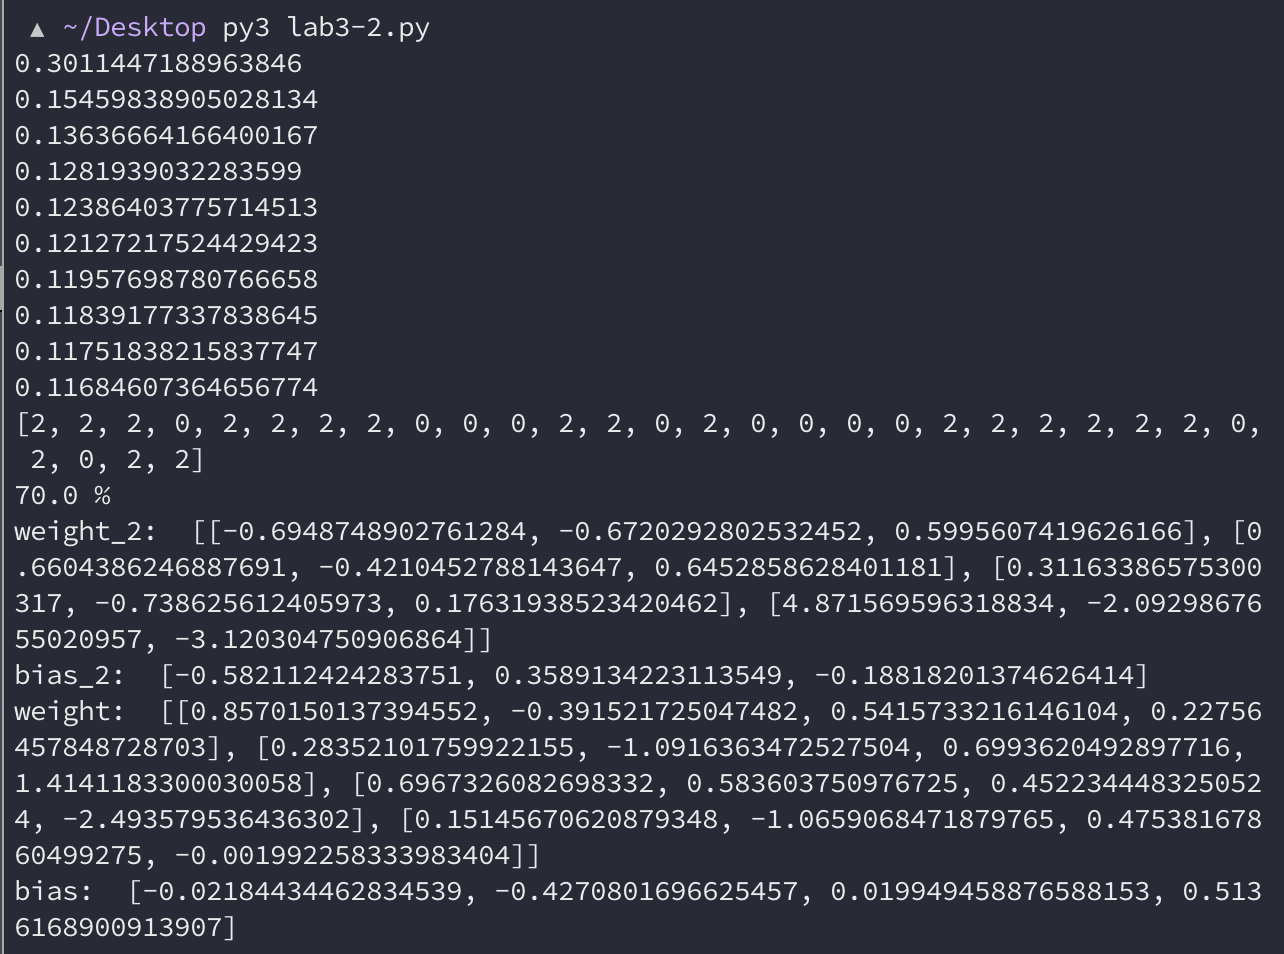
\includegraphics[scale=0.65]{ot2.png}\\
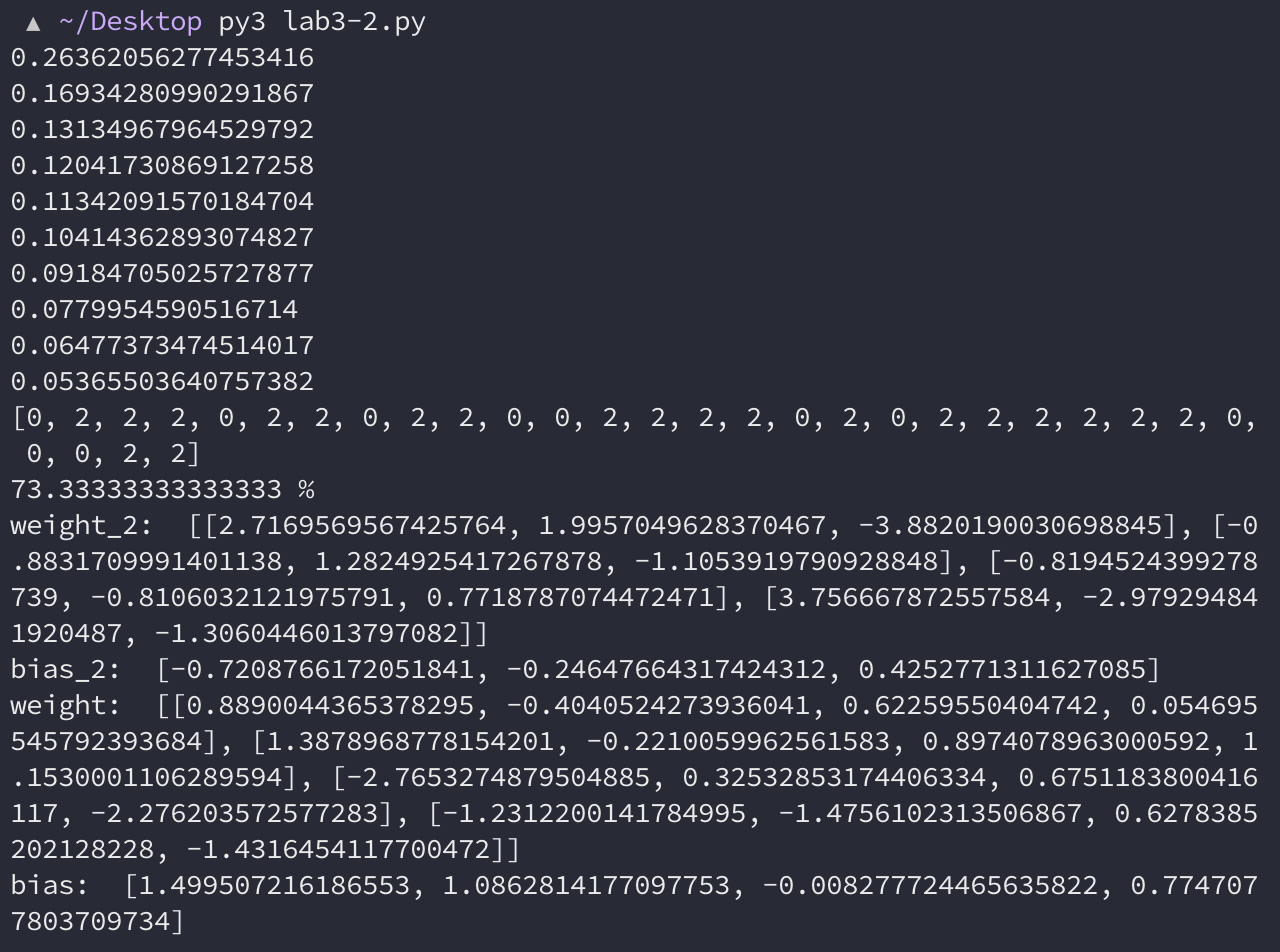
\includegraphics[scale=0.65]{ot3.png}\\
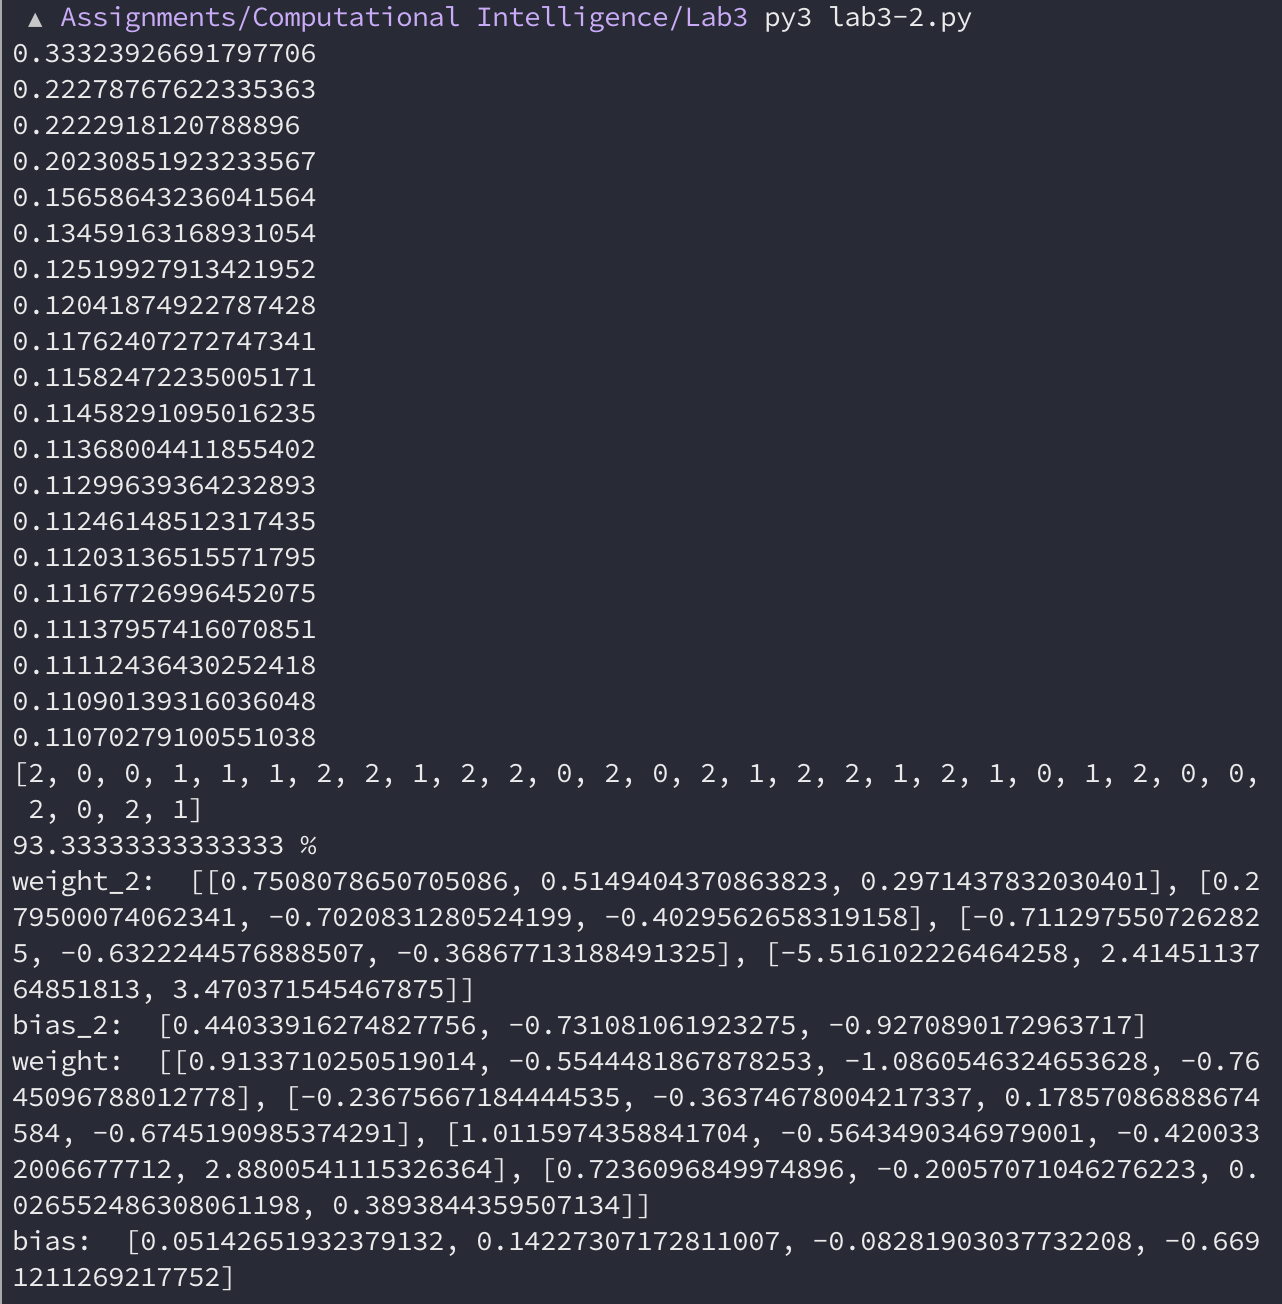
\includegraphics[scale=0.65]{ot4.png}


\end{document}
